\documentclass[journal,12pt,twocolumn]{IEEEtran}

\usepackage{setspace}
\usepackage{gensymb}
\singlespacing
\usepackage[cmex10]{amsmath}

\usepackage{amsthm}

\usepackage{mathrsfs}
\usepackage{txfonts}
\usepackage{stfloats}
\usepackage{bm}
\usepackage{cite}
\usepackage{cases}
\usepackage{subfig}

\usepackage{longtable}
\usepackage{multirow}

\usepackage{enumitem}
\usepackage{mathtools}
\usepackage{steinmetz}
\usepackage{tikz}
\usepackage{circuitikz}
\usepackage{verbatim}
\usepackage{tfrupee}
\usepackage[breaklinks=true]{hyperref}
\usepackage{graphicx}
\usepackage{tkz-euclide}

\usetikzlibrary{calc,math}
\usepackage{listings}
    \usepackage{color}                                            %%
    \usepackage{array}                                            %%
    \usepackage{longtable}                                        %%
    \usepackage{calc}                                             %%
    \usepackage{multirow}                                         %%
    \usepackage{hhline}                                           %%
    \usepackage{ifthen}                                           %%
    \usepackage{lscape}     
\usepackage{multicol}
\usepackage{chngcntr}
\setcounter{MaxMatrixCols}{20}

\DeclareMathOperator*{\Res}{Res}

\renewcommand\thesection{\arabic{section}}
\renewcommand\thesubsection{\thesection.\arabic{subsection}}
\renewcommand\thesubsubsection{\thesubsection.\arabic{subsubsection}}

\renewcommand\thesectiondis{\arabic{section}}
\renewcommand\thesubsectiondis{\thesectiondis.\arabic{subsection}}
\renewcommand\thesubsubsectiondis{\thesubsectiondis.\arabic{subsubsection}}


\hyphenation{op-tical net-works semi-conduc-tor}
\def\inputGnumericTable{}                                 %%

\lstset{
%language=C,
frame=single, 
breaklines=true,
columns=fullflexible
}
\begin{document}


\newtheorem{theorem}{Theorem}[section]
\newtheorem{problem}{Problem}
\newtheorem{proposition}{Proposition}[section]
\newtheorem{lemma}{Lemma}[section]
\newtheorem{corollary}[theorem]{Corollary}
\newtheorem{example}{Example}[section]
\newtheorem{definition}[problem]{Definition}

\newcommand{\BEQA}{\begin{eqnarray}}
        \newcommand{\EEQA}{\end{eqnarray}}
\newcommand{\define}{\stackrel{\triangle}{=}}
\bibliographystyle{IEEEtran}
\raggedbottom
\setlength{\parindent}{0pt}
\providecommand{\mbf}{\mathbf}
\providecommand{\pr}[1]{\ensuremath{\Pr\left(#1\right)}}
\providecommand{\qfunc}[1]{\ensuremath{Q\left(#1\right)}}
\providecommand{\sbrak}[1]{\ensuremath{{}\left[#1\right]}}
\providecommand{\lsbrak}[1]{\ensuremath{{}\left[#1\right.}}
\providecommand{\rsbrak}[1]{\ensuremath{{}\left.#1\right]}}
\providecommand{\brak}[1]{\ensuremath{\left(#1\right)}}
\providecommand{\lbrak}[1]{\ensuremath{\left(#1\right.}}
\providecommand{\rbrak}[1]{\ensuremath{\left.#1\right)}}
\providecommand{\cbrak}[1]{\ensuremath{\left\{#1\right\}}}
\providecommand{\lcbrak}[1]{\ensuremath{\left\{#1\right.}}
\providecommand{\rcbrak}[1]{\ensuremath{\left.#1\right\}}}
\theoremstyle{remark}
\newtheorem{rem}{Remark}
\newcommand{\sgn}{\mathop{\mathrm{sgn}}}
\providecommand{\abs}[1]{\left\vert#1\right\vert}
\providecommand{\res}[1]{\Res\displaylimits_{#1}}
\providecommand{\norm}[1]{\left\lVert#1\right\rVert}
%\providecommand{\norm}[1]{\lVert#1\rVert}
\providecommand{\mtx}[1]{\mathbf{#1}}
\providecommand{\mean}[1]{E\left[ #1 \right]}
\providecommand{\fourier}{\overset{\mathcal{F}}{ \rightleftharpoons}}
%\providecommand{\hilbert}{\overset{\mathcal{H}}{ \rightleftharpoons}}
\providecommand{\system}{\overset{\mathcal{H}}{ \longleftrightarrow}}
%\newcommand{\solution}[2]{\textbf{Solution:}{#1}}
\newcommand{\solution}{\noindent \textbf{Solution: }}
\newcommand{\cosec}{\,\text{cosec}\,}
\providecommand{\dec}[2]{\ensuremath{\overset{#1}{\underset{#2}{\gtrless}}}}
\newcommand{\myvec}[1]{\ensuremath{\begin{pmatrix}#1\end{pmatrix}}}
\newcommand{\mydet}[1]{\ensuremath{\begin{vmatrix}#1\end{vmatrix}}}
\numberwithin{equation}{subsection}
\makeatletter
\@addtoreset{figure}{problem}
\makeatother
\let\StandardTheFigure\thefigure
\let\vec\mathbf
\renewcommand{\thefigure}{\theproblem}
\def\putbox#1#2#3{\makebox[0in][l]{\makebox[#1][l]{}\raisebox{\baselineskip}[0in][0in]{\raisebox{#2}[0in][0in]{#3}}}}
\def\rightbox#1{\makebox[0in][r]{#1}}
\def\centbox#1{\makebox[0in]{#1}}
\def\topbox#1{\raisebox{-\baselineskip}[0in][0in]{#1}}
\def\midbox#1{\raisebox{-0.5\baselineskip}[0in][0in]{#1}}
\vspace{3cm}
\title{EE4013 Assignment-1}
\author{PEDAVEGI ADITYA - EE18BTECH11034}
\maketitle
\newpage
\bigskip
\renewcommand{\thefigure}{\theenumi}
\renewcommand{\thetable}{\theenumi}
Download all the codes from
\begin{lstlisting}
https://github.com/adi2000pedavegi/EE4013/tree/main/Assignment-1/codes
\end{lstlisting}
%
and latex-tikz codes from
%
\begin{lstlisting}
https://github.com/adi2000pedavegi/EE4013/tree/main/Assignment-1/figs
\end{lstlisting}
\section{Problem}
Consider the following C program
\begin{lstlisting}
#include <stdio.h>
int main ()
{
	int arr[] = {1,2,3,4,5,6,7,8,9,0,1,2,5}, *ip = arr + 4;
	printf("%d\n",ip[1]);
	return 0;
}

\end{lstlisting}
The number that will be dispalyed on the execution of the program is :
\section{Solution}
The output of the given C program is
\begin{lstlisting}
    6
\end{lstlisting}

Initially we defined an integer array by name $arr$ of size 13.
\begin{lstlisting}
    int arr[] = {1,2,3,4,5,6,7,8,9,0,1,2,5};
\end{lstlisting}


An array in C or be it in any programming language is a collection of
similar data items stored at contiguous memory locations and elements can be
accessed randomly using indices of an array. They can be used to store
collection of primitive data types such as int, float, double, char, etc of any
particular type.

The created array will be created as shown in Fig.\ref{fig:ee18btech11034_1}
\begin{figure}[!ht]
    \begin{center}
        \resizebox{\columnwidth}{!}{%\begin{figure}


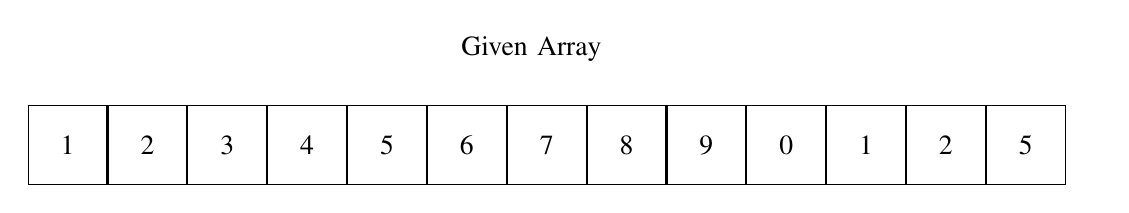
\begin{tikzpicture}[auto, node distance=3cm,>=latex']
    \node [draw,
        minimum width=1cm,
        minimum height=1cm
    ]  (Element1) at (0,0) {$1$};
    \node [draw,
        minimum width=1cm,
        minimum height=1cm,
        right=0cm of Element1
    ]  (Element2) {$2$};
    \node [draw,
        minimum width=1cm,
        minimum height=1cm,
        right=0cm of Element2
    ]  (Element3) {$3$};
    \node [draw,
        minimum width=1cm,
        minimum height=1cm,
	right=0cm of Element3
    ]  (Element4) {$4$};
    \node [draw,
        minimum width=1cm,
        minimum height=1cm,
        right=0cm of Element4
    ]  (Element5) {$5$};
    \node [draw,
        minimum width=1cm,
        minimum height=1cm,
        right=0cm of Element5
    ]  (Element6) {$6$};
    \node [draw,
        minimum width=1cm,
        minimum height=1cm,
	right=0cm of Element6
    ]  (Element7) {$7$};
    \node [draw,
        minimum width=1cm,
        minimum height=1cm,
        right=0cm of Element7
    ]  (Element8) {$8$};
    \node [draw,
        minimum width=1cm,
        minimum height=1cm,
        right=0cm of Element8
    ]  (Element9) {$9$};
    \node [draw,
        minimum width=1cm,
        minimum height=1cm,
	right=0cm of Element9
    ]  (Element10) {$0$};
    \node [draw,
        minimum width=1cm,
        minimum height=1cm,
        right=0cm of Element10
    ]  (Element11) {$1$};
    \node [draw,
        minimum width=1cm,
        minimum height=1cm,
        right=0cm of Element11
    ]  (Element12) {$2$};
    \node [draw,
        minimum width=1cm,
        minimum height=1cm,
        right=0cm of Element12
    ]  (Element13) {$5$};

    \node[text width=8cm, anchor=north] at (9,1.5)
    {Given Array};

\end{tikzpicture}
%\end{figure
}
    \end{center}
    \caption{Given Input array}
    \label{fig:ee18btech11034_1}
\end{figure}

By default while creating an array, a pointer as the name of the array i.e., $arr$ is
created and it stores the address of the first element in the arr.

This is shown in below Fig.\ref{fig:ee18btech11034_2}

Then we initialized a pointer $ip$ as
\begin{lstlisting}
    int *ip = arr + 4;
\end{lstlisting}
The above line of code creates a pointer such that it points to the $4^{th}$ element from the
element pointed by pointer $arr$ i.e., the pointer $ip$ stores the address of the element
present in $5^{th}$ index of array arr. This is pictured in Fig.\ref{fig:ee18btech11034_2}
\begin{figure}[!ht]
    \begin{center}
        \resizebox{\columnwidth}{!}{%\begin{figure}


% The block diagram code is probably more verbose than necessary
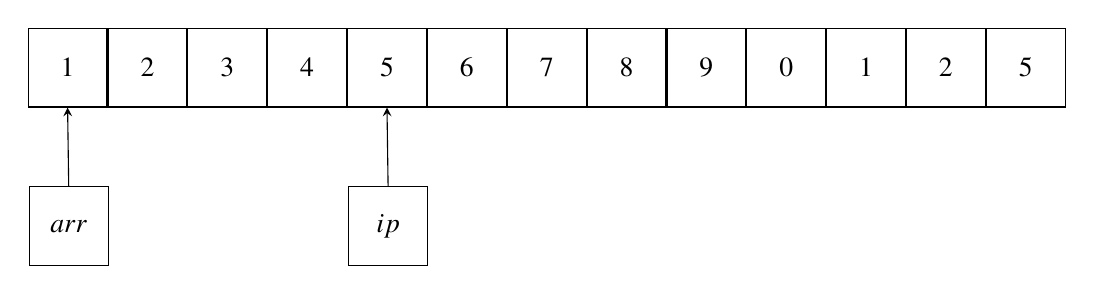
\begin{tikzpicture}[auto, node distance=3cm,>=latex']
    % Controller
    \node [draw,
        minimum width=1cm,
        minimum height=1cm
    ]  (Element1) at (0,0) {$1$};
    \node [draw,
        minimum width=1cm,
        minimum height=1cm,
        right=0cm of Element1
    ]  (Element2) {$2$};
    \node [draw,
        minimum width=1cm,
        minimum height=1cm,
        right=0cm of Element2
    ]  (Element3) {$3$};
    % Controller
    \node [draw,
        minimum width=1cm,
        minimum height=1cm,
	right=0cm of Element3
    ]  (Element4) {$4$};
    \node [draw,
        minimum width=1cm,
        minimum height=1cm,
        right=0cm of Element4
    ]  (Element5) {$5$};
    \node [draw,
        minimum width=1cm,
        minimum height=1cm,
        right=0cm of Element5
    ]  (Element6) {$6$};
    % Controller
    \node [draw,
        minimum width=1cm,
        minimum height=1cm,
	right=0cm of Element6
    ]  (Element7) {$7$};
    \node [draw,
        minimum width=1cm,
        minimum height=1cm,
        right=0cm of Element7
    ]  (Element8) {$8$};
    \node [draw,
        minimum width=1cm,
        minimum height=1cm,
        right=0cm of Element8
    ]  (Element9) {$9$};
    % Controller
    \node [draw,
        minimum width=1cm,
        minimum height=1cm,
	right=0cm of Element9
    ]  (Element10) {$0$};
    \node [draw,
        minimum width=1cm,
        minimum height=1cm,
        right=0cm of Element10
    ]  (Element11) {$1$};
    \node [draw,
        minimum width=1cm,
        minimum height=1cm,
        right=0cm of Element11
    ]  (Element12) {$2$};
    \node [draw,
        minimum width=1cm,
        minimum height=1cm,
        right=0cm of Element12
    ]  (Element13) {$5$};

    \node[draw,
	minimum width=1cm,
	minimum height=1cm,
	below right = 1cm and -1cm of Element1
    ]  (PointerArr) {$arr$};
    \draw[-stealth] (PointerArr.north) -- (Element1.south)
    node[midway,above]{};
    \node[draw,
	minimum width=1cm,
	minimum height=1cm,
	below right = 1cm and -1cm of Element5
    ]  (PointerIp) {$ip$};
    \draw[-stealth] (PointerIp.north) -- (Element5.south)
    node[midway,above]{};
    
\end{tikzpicture}
%\end{figure
}
    \end{center}
    \caption{Pointer pointing to an element in array}
    \label{fig:ee18btech11034_2}
\end{figure}

Now the final line of code is:
\begin{lstlisting}
    printf("%d\n",ip[1]);
\end{lstlisting}

Using this line of code we are printing the element present in $ip[1]$. The value of
$ip[1]$ i.e $(^{*}(ip+1))$ is equivalent to element present in memory address pointed by the pointer
$ip+1$.

The element pointed by pointer $ip+1$ is shown in Fig. \ref{fig:ee18btech11034_3}

\begin{figure}[!ht]
    \begin{center}
        \resizebox{\columnwidth}{!}{%\begin{figure}


% The block diagram code is probably more verbose than necessary
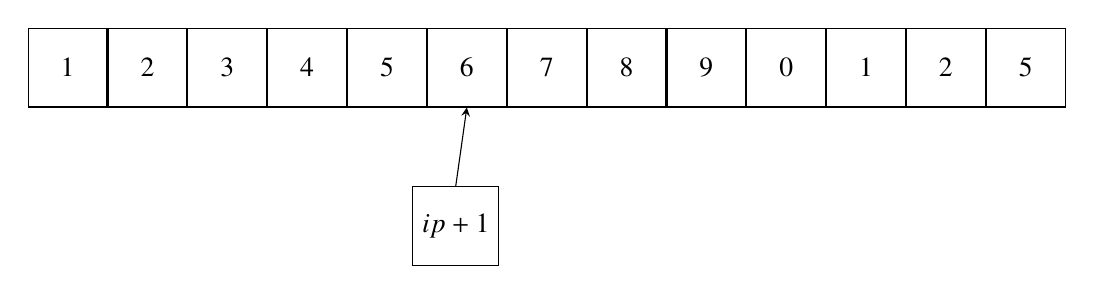
\begin{tikzpicture}[auto, node distance=3cm,>=latex']
    % Controller
    \node [draw,
        minimum width=1cm,
        minimum height=1cm
    ]  (Element1) at (0,0) {$1$};
    \node [draw,
        minimum width=1cm,
        minimum height=1cm,
        right=0cm of Element1
    ]  (Element2) {$2$};
    \node [draw,
        minimum width=1cm,
        minimum height=1cm,
        right=0cm of Element2
    ]  (Element3) {$3$};
    % Controller
    \node [draw,
        minimum width=1cm,
        minimum height=1cm,
	right=0cm of Element3
    ]  (Element4) {$4$};
    \node [draw,
        minimum width=1cm,
        minimum height=1cm,
        right=0cm of Element4
    ]  (Element5) {$5$};
    \node [draw,
        minimum width=1cm,
        minimum height=1cm,
        right=0cm of Element5
    ]  (Element6) {$6$};
    % Controller
    \node [draw,
        minimum width=1cm,
        minimum height=1cm,
	right=0cm of Element6
    ]  (Element7) {$7$};
    \node [draw,
        minimum width=1cm,
        minimum height=1cm,
        right=0cm of Element7
    ]  (Element8) {$8$};
    \node [draw,
        minimum width=1cm,
        minimum height=1cm,
        right=0cm of Element8
    ]  (Element9) {$9$};
    % Controller
    \node [draw,
        minimum width=1cm,
        minimum height=1cm,
	right=0cm of Element9
    ]  (Element10) {$0$};
    \node [draw,
        minimum width=1cm,
        minimum height=1cm,
        right=0cm of Element10
    ]  (Element11) {$1$};
    \node [draw,
        minimum width=1cm,
        minimum height=1cm,
        right=0cm of Element11
    ]  (Element12) {$2$};
    \node [draw,
        minimum width=1cm,
        minimum height=1cm,
        right=0cm of Element12
    ]  (Element13) {$5$};

    
    \node[draw,
	minimum width=1cm,
	minimum height=1cm,
	below right = 1cm and -1.2cm of Element6
    ]  (PointerIp) {$ip+1$};
    \draw[-stealth] (PointerIp.north) -- (Element6.south)
    node[midway,above]{};
    
\end{tikzpicture}
%\end{figure
}
    \end{center}
    \caption{}
    \label{fig:ee18btech11034_3}
\end{figure}

So, now the above printf line prints the integer stored at the address, the pointer $ip+1$
points in the terminal i.e., \textbf{6}.

\section{Vector Form Approach}
Consider the given array as a vector $arr$, multiplying it with another vector of same length having 0's and 1's. 
The other vector have 0's at all indexes except at the required index.
\\
Consider the identity matrix I of size $nxn$
\\
\[I = 
	\begin{bmatrix}
		1 & 0 & 0 & 0 & . & . & . & 0 & 0 & 0
		\\
		0 & 1 & 0 & 0 & . & . & . & 0 & 0 & 0
		\\
		0 & 0 & 1 & 0 & . & . & . & 0 & 0 & 0
		\\
		. & . & . & . & . & . & . & . & . & .
		\\
		0 & 0 & 0 & 0 & . & . & . & 0 & 1 & 0
		\\
		0 & 0 & 0 & 0 & . & . & . & 0 & 0 & 1
	\end{bmatrix}
\]
The eigen vectors of the above I matrix gives $n$ unit vectors $e_{0}$ to $e_{n-1}$ each of size $nx1$ where
\\

$$
	e_{0} = 
	\begin{bmatrix}
		1
		\\
		0
		\\
		0
		\\
		.
		\\
		.
		\\
		0
	\end{bmatrix}
	e_{1} = 
	\begin{bmatrix}
		0
		\\
		1
		\\
		0
		\\
		.
		\\
		.
		\\
		0
	\end{bmatrix}
	.......
	e_{n-1} = 
	\begin{bmatrix}
		0
		\\
		0
		\\
		0
		\\
		.
		\\
		.
		\\
		1
	\end{bmatrix}
$$
\\
Hence the column unit vector $e_{i}$ has value 1 at ith place (index) and 0's at other indexes. 
\\
The given pointer $ip$ gives the 4th index in $arr$.So the value $ip[1]$ i.e $(^{*}(ip+1))$ gives the 5th index in $arr$ i.e $\textbf{arr[5]}$
\\
Element wise multiplication (inner product) of two vectors $arr$ and $e_{5}$ gives the required output.
\\
\begin{align}
arr[i] = arr^{T}e_{i}
\end{align}
So 
\begin{align}
arr[5] = arr^{T}e_{5}
\end{align}
\\
\[
	arr = 
	\begin{bmatrix}
		1 
		\\
		2
		\\
		3
		\\
		4
		\\
		5
		\\
		6
		\\
		7
		\\
		8
		\\
		9
		\\
		0
		\\
		1
		\\
		2
		\\
		5
	\end{bmatrix}
\]
$$
	e_{5} = 
	\begin{bmatrix}
		0
		\\
		0
		\\
		0
		\\
		0
		\\
		0
		\\
		1
		\\
		0
		\\
		0
		\\
		0
		\\
		0
		\\
		0
		\\
		0
		\\
		0
	\end{bmatrix}
$$
\\
Vector multiplication of $arr$ and $e_{5}$ i.e $arr^{T}e_{5}$ gives \\
\[
	\begin{bmatrix}
		1 & 2 & 3 & 4 & 5 & 6 & 7 & 8 & 9 & 0 & 1 & 2 & 5
	\end{bmatrix}
	\begin{bmatrix}
		0
		\\
		0
		\\
		0
		\\
		0
		\\
		0
		\\
		1
		\\
		0
		\\
		0
		\\
		0
		\\
		0
		\\
		0
		\\
		0
		\\
		0
	\end{bmatrix}
\]
=
\[
	\begin{bmatrix}
	6 
	\end{bmatrix}
\]
\end{document}
